\chapter{Comunicazione tra processi}

Normalmente i processi si dividono in processi indipendenti, ovvero quei processi la cui esecuzione è indipendente da quella degli altri processi ed non condivide i dati, e processi cooperanti, ovvero quei processi che condividono i dati e devono comunicare tra loro, la loro esecuzione non è deterministica e non è riproducibile.
\paragraph{In generale}
    Esistono diversi motivi per cui i processi devono comunicare tra loro, tra cui:
    \begin{itemize}
        \item \textbf{Scambio di informazioni}: i processi devono scambiarsi informazioni per cooperare tra loro.
        \item \textbf{Accelerazione del calcolo}: i processi possono cooperare per eseguire un calcolo più velocemente.
        \item \textbf{Modularità}: i processi possono essere scritti in modo indipendente e comunicare tra loro per cooperare.
        \item \textbf{Convenienza}: è più semplice scrivere processi separati che cooperano tra loro piuttosto che scrivere un unico processo.
    \end{itemize}
    per ottenere una comunicazione tra processi è necessario che i processi condividano un canale di comunicazione, esistono due tipi di canali di comunicazione:
    \begin{description}
        \item[scambio di messaggi] i processi comunicano scambiandosi messaggi che vengono inviati attraverso un canale di comunicazione tra il \textit{kernel} e i processi, i messaggi possono essere inviati in modo sincrono o asincrono.
        \item[memoria condivisa] i processi comunicano condividendo una regione di memoria, i processi possono leggere e scrivere nella memoria condivisa, la memoria condivisa è un canale di comunicazione molto più veloce rispetto allo scambio di messaggi, ma è più difficile da gestire.
    \end{description}
    Il primo risulta più sicuro in quanto i processi non possono accedere direttamente alla memoria degli altri processi ed il messaggio viene verificato dal \textit{kernel} prima di essere inviato, mentre il secondo è più veloce in quanto non richiede l'intervento del \textit{kernel} per la comunicazione.\newline
    Tutti i meccanismi di comunicazione tra processi sono implementati dal \textit{kernel} del sistema operativo racchiusi nei protocolli di comunicazione tra processi (\texttt{IPC} - \textit{Inter-Process Communication}).

\section{\texttt{IPC} - \textit{Message Passing}}
    Il protocollo \texttt{ICP} racchiude un insieme di meccanismi che permettono la comunicazione tra processi, tra i quali vi è il \textit{message passing}, ovvero un meccanismo che permette ai processi di comunicare scambiandosi messaggi e senza condividere delle variabili e/o memoria. Le operazioni di base che ogni \texttt{SO} deve fornire per il \textit{message passing} sono:
    \begin{itemize}
        \item \texttt{send} - invia un messaggio ad un processo. (con lunghezza fissa o variabile)
        \item \texttt{receive} - riceve un messaggio da un processo.
    \end{itemize}
    Prima ancora che i processi possano comunicare tra loro è necessario che essi siano in grado di identificarsi e stabilire un canale di comunicazione, per fare ciò è necessario che i processi abbiano un identificativo univoco, ovvero un \textit{PID} (\textit{Process IDentifier}).\newline
    L'implementazione di questo canale di comunicazione può essere realizzata in due modi:
    \begin{description}
        \item[livello fisico] i messaggi vengono inviati attraverso un canale di comunicazione fisico, come ad esempio una rete o un bus.
        \item[livello logico] i messaggi vengono inviati attraverso un canale di comunicazione logico, come ad esempio una coda di messaggi.
    \end{description}
    Le scelte di uno o dell'altro canale di comunicazione dipendono dalle esigenze del sistema e dalle prestazioni richieste. Fattori che influenzano la scelta sono:
    \begin{itemize}
        \item Come vengono stabiliti i canali
        \item Se un canale può essere utilizzato da più processi contemporaneamente
        \item Quanti canali possono essere aperti contemporaneamente tra una stessa coppia di processi
        \item La lunghezza massima del canale
        \item La lunghezza (fissa/variabile) massima dei messaggi
        \item Se il canale è \textit{simplex}, \textit{half-duplex} o \textit{full-duplex}
    \end{itemize}
    \subsection{Nominazione}
        A livello di nominazione, ovvero come i processi si identificano, esiste la comunicazione diretta e la comunicazione indiretta:
        \subsubsection{Comunicazione Diretta}
            Nella comunicazione diretta i processi si identificano direttamente, ovvero il mittente conosce l'identificativo del destinatario e viceversa, in questo modo il mittente può inviare il messaggio direttamente al destinatario. Questo metodo è molto veloce, ma presenta dei problemi:
            \begin{itemize}
                \item Il mittente deve conoscere l'identificativo del destinatario
                \item Il destinatario deve essere in esecuzione
                \item Nel caso in cui il destinatario o il ricevente cambi identificativo, il mittente deve essere aggiornato
            \end{itemize}
            La comunicazione diretta può a sua volta essere simmetrica o asimmetrica:
            \begin{description}
                \item[Simmetrica] Il mittente e il destinatario si conoscono a priori e possono comunicare tra loro. Sia per l'invio che per la ricezione dei messaggi è necessario conoscere l'identificativo del processo con cui si vuole comunicare.
                \item[Asimmetrica] Il mittente e il destinatario non si conoscono a priori. Solo il mittente conosce l'identificativo del destinatario, il destinatario non conosce l'identificativo del mittente ed ascolta qualsiasi messaggio che arriva.
            \end{description}
        \subsubsection{Comunicazione Indiretta}
            Nella comunicazione indiretta i messaggi vengono inviati ad un canale di comunicazione comune detto \textit{mailbox} (o porte), ognuna di queste \textit{mailbox} ha associato un numero identificativo univoco, i processi possono inviare e ricevere messaggi da queste \textit{mailbox} senza dover conoscere l'identificativo del destinatario, ma devono condividere una \textit{mailbox} comune.
            \paragraph{Flusso di una \textit{mailbox}}
                Prima di poter inviare un messaggio ad una \textit{mailbox} è necessario che questa venga creata, una volta creata la \textit{mailbox} il processo può inviare un messaggio ad essa, il messaggio viene inserito in una coda di messaggi associata alla \textit{mailbox}, il destinatario può ricevere il messaggio dalla \textit{mailbox} e leggerlo, una volta letto il messaggio viene rimosso dalla coda. Quando la \textit{mailbox} non è più necessaria può essere eliminata.
            \paragraph{Invio e ricezione} 
                Per inviare e ricevere messaggi da una \textit{mailbox} è necessario conoscere l'identificativo della \textit{mailbox}, una volta conosciuto l'identificativo il processo può inviare e ricevere messaggi dalla \textit{mailbox}.
            \paragraph{Proprietà del canale} Come già detto, il canale di comunicazione viene stabilito solo se i processi condividono una \textit{mailbox}, ma una \textit{mailbox} può essere associata a molti processi ed una stessa coppia di processi può avere più \textit{mailbox} associate, inoltre una \textit{mailbox} può essere o meno bi-direzionale.
            \paragraph{Problema riceventi multipli} Un problema che si può presentare è quello dei riceventi multipli, ovvero quando un mittente invia un messaggio ad una \textit{mailbox} e ci sono più processi che ricevono i messaggi da quella \textit{mailbox}, in questo caso il \textit{SO} deve permettere solo ad uno dei processi di ricevere il messaggio, e questo viene fatto in maniera arbitraria.
    \subsection{Sincronizzazione} 
        Uno scambio di messaggi può essere ``bloccante'' (sincrono) o ``non bloccante'' (asincrono), ovvero il mittente può continuare ad eseguire il proprio codice dopo aver inviato il messaggio o deve attendere che il destinatario riceva il messaggio.\newline
        Se il canale di comunicazione è bloccante, il mittente deve attendere che il destinatario riceva il messaggio ed assicurarsi che il messaggio sia stato ricevuto, se il canale di comunicazione è non bloccante il mittente può continuare ad eseguire il proprio codice dopo aver inviato il messaggio, senza dover attendere che il destinatario riceva il messaggio, in questo caso il mittente non può sapere se il messaggio è stato ricevuto o meno.
        \begin{figure}[H]
            \begin{subfigure}{0.45\textwidth}
                \centering
                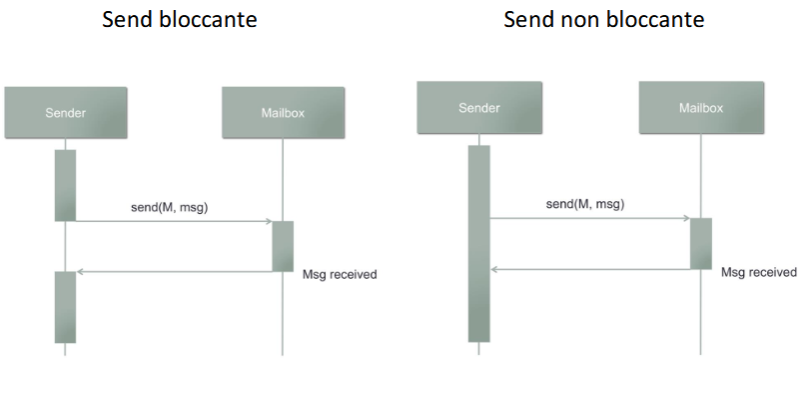
\includegraphics[width=\textwidth]{05/send.png}
                \caption{Invio bloccante/non bloccante}
            \end{subfigure}
            \begin{subfigure}{0.45\textwidth}
                \centering
                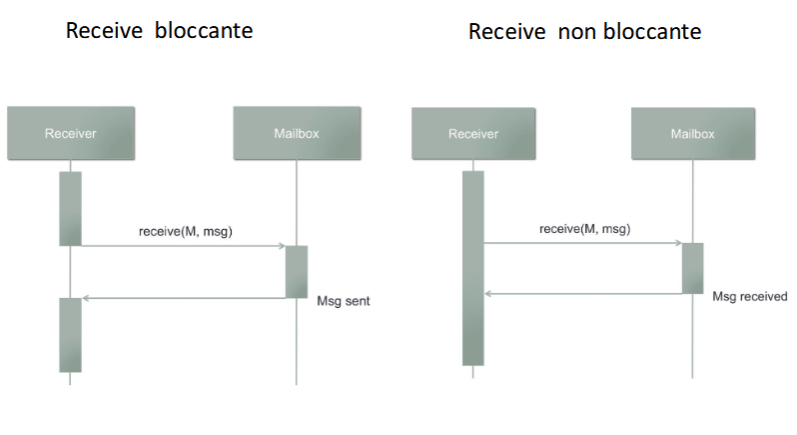
\includegraphics[width=\textwidth]{05/receive.png}
                \caption{Ricezione bloccante/non bloccante}
            \end{subfigure}
            \caption{Invio e ricezione bloccante/non bloccante}
        \end{figure}

\section{\texttt{IPC} - Memoria Condivisa}
    Un altro meccanismo di comunicazione tra processi è la memoria condivisa, ovvero un'area di memoria condivisa tra più processi, i processi possono leggere e scrivere nella memoria condivisa, la memoria condivisa è un canale di comunicazione molto più veloce rispetto allo scambio di messaggi, ma è più difficile da gestire, inoltre il \textit{kernel} non può controllare l'accesso alla memoria condivisa, quindi è necessario che i processi si sincronizzino tra loro per evitare problemi di accesso concorrente.
    \subsubsection{Flusso di \texttt{POSIX}}
        Prendiamo come esempio la memoria condivisa in \texttt{POSIX}, per poter utilizzare la memoria condivisa è necessario che uno dei processi crei la memoria condivisa, una volta creata la memoria condivisa l'altro processo deve ``attaccarsi'' al segmento di memoria condivisa, una volta ``attaccato'' il processo può avere il permesso di leggere e scrivere oppure solo di leggere, una volta terminato il processo deve ``staccarsi'' dalla memoria condivisa. Il processo che ha creato la memoria condivisa deve rimuoverla una volta terminato.
    \subsubsection{Le \textit{pipe}}
        Un altro meccanismo di comunicazione tra processi è la \textit{pipe}, ovvero un canale di comunicazione tra processi. \newline
        La \textit{pipe} è un canale di comunicazione che permette di inviare e ricevere messaggi tra processi, la \textit{pipe} è un canale di comunicazione unidirezionale, ovvero i messaggi possono essere inviati in una sola direzione, ma è possibile creare due \textit{pipe} per permettere la comunicazione in entrambe le direzioni. Distinguiamo tra \textit{pipe} ordinarie e \textit{pipe} con nome:
        \paragraph{\textit{Pipe} ordinarie} Le \textit{pipe} ordinarie permettono la comunicazione in uno stile ``Produttore-Consumatore'' dove il produttore scrive nella \textit{pipe} e il consumatore legge dalla \textit{pipe}, questa tipologia richiede una relazione tra processi, queste infatti possono essere aperte solo da processi padri verso i processi figli.
        \paragraph{\textit{Pipe} con nome} Le \textit{pipe} con nome sono simili alle \textit{pipe} ordinarie, ma permettono la comunicazione bidirezionale, non è richiesta la relazione tra processi e più processi possono usare la stessa \textit{pipe} per comunicare tra loro, ma è necessario che i processi si sincronizzino tra loro per evitare problemi di accesso concorrente. Le \textit{pipe} con nome sono disponibili sia in sistemi \texttt{UNIX} che in sistemi \texttt{Windows}, ma in quest'ultimo caso non sono implementate come file di tipo \textit{FIFO} ma come file temporanei.